% $Id$
%==============================================================================
\section{CORBA Component Model (CCM)}
%==============================================================================

Developing CORBA applications that make use of advanced features of the 
ORB and rely on services such as security, notification, persistent state
and transactions requires a substantial development effort.
The OMG addresses these problems by introducing the concept of CORBA components.

%==============================================================================
\subsection{CORBA Component definition}
%==============================================================================
\begin{description} 
\item [CCM Component Definition:]
A component is a basic meta--type in CORBA 3.0 and is denoted by a component
reference.
A component type is a specific, named collection of features that can be
described by an IDL component definition.
A component type encapsulates its internal representation and implementation.
\end{description}

\begin{figure}[htbp]
    \begin{center}
    \includegraphics [height=4cm,angle=0] {figures/CCMSymbol.eps}
    \caption{Pictorial representation of a CCM component that supports a {\tt Home}
    and an {\tt Equivalent} interface as well as synchronous (facet, receptacle)
    and asynchronous ports (event source, event sink).}
    \label{ComponentAndContainer}            
    \end{center}
\end{figure}

\noindent
CCM defines a component 
architecture and a container framework in which the component life cycle takes
place. 
In the CCM specification \cite{CCMSpecification}, the following component 
types are defined:
\begin{description}
\item {\bf Service Components} do not have any state. The lifetime of service
components is restricted to the lifetime of a single method call.
A service component is equivalent to a stateless EJB session bean.

\item {\bf Session Components} have transient state. Typically, a session 
component will have the lifetime of a client interaction.
Session components are equivalent to stateful EJB session beans.

\item {\bf Process Components} have persistent state but no primary key.
They are used to model business processes, usually tasks with a well--defined
lifetime.

\item {\bf Entity Components} have persistent state and a primary key.
They are used to model persistent entities in a database that may have 
transactional behavior.
CCM defines two forms of persistence support:
	\begin{itemize}
	\item {\bf Container--managed Persistence} (CMP): 
	The component developer simply defines the state that is to be made 
	persistent and the container automatically saves and restores state 
	as required.
	\item {\bf Self--managed Persistence} (SMP): 
	The component developer assumes the responsibility for saving and 
	restoring state when requested to do so by the container.
	\end{itemize}	
\end{description}

\vspace{3mm}
\noindent
The external view of a CCM component (Fig.~\ref{ComponentAndContainer}) 
is defined by the following interfaces:

\begin{itemize}
\item {\bf Component Home Interface:} describes an interface for managing 
instances
of a specific component type.
The home interface may define {\it Factory Methods} and {\it Finder Methods} to 
create and retrieve component instances.
A home definition can optionally have {\it Supported Interfaces} that means that
the home interface inherits from these interfaces.

\item {\bf Component Equivalent Interface:} is the component's main interface.
{\it Attributes} and {\it Supported Interfaces} are included in the equivalent
interface as well as navigation methods to access the component's ports. 

\item {\bf Provided Interfaces:} a component type may provide several 
implemented interfaces to its clients in the form of {\it Facets}.
Facets are intended to be the primary vehicle through which a component exposes
its functional application behavior to clients during normal execution.
Provided interfaces follow the concept introduced by the 
{\it Extension Interface} pattern \cite{POSA2}.

\item {\bf Used Interfaces:} a component definition can describe the ability
to use object references upon which the component may invoke operations.
When a component accepts an object reference in this manner, the relationship
between the component and the referent object is called a connection.
The conceptional point of connection is called a {\it Receptacle}.
\end{itemize}

\noindent
In addition to the presented interfaces, CCM supports a publish/subscribe event 
model.
{\bf Event Sources} hold references to consumer interfaces and invoke various 
forms of push operations to send events.
Component {\bf Event Sinks} provide consumer references, into which other 
entities push events.
An {\it Emitter} can be connected to at most one provider, while a 
{\it Publisher} can be connected to an arbitrary number of consumers.
The possible dependencies between these interfaces are defined in the CCM 
{\bf Interface Repository Metamodel}.

\vspace{3mm}
\noindent
All interfaces of a CORBA component are described in the OMG 
{\bf Interface Definition Language} (IDL) which is part of the CORBA 3.0 
specification.
The use of IDL makes the component definition independent of programming 
languages.
The OMG has defined language mappings that describe the realization of IDL 
constructs in a particular programming language.

\vspace{3mm}
\noindent
To describe the structure and state of component implementations, the OMG 
defined the {\bf Component Implementation Definition Language} (CIDL) as a 
superset of the {\it Persistent State Definition Language}.
The {\bf Component Implementation Framework} (CIF) defines the programming model
for constructing component implementations.
The CIF uses CIDL descriptions to generate programming skeletons that automate
many of the basic behaviors of components.

%==============================================================================
\subsection{CORBA Component Container}
%==============================================================================
The CCM architecture (Fig.~\ref{CCMArchitecture}) is very similar to EJB.
Components run in a {\bf CCM Container} that provides the runtime environment 
for CORBA components.

\begin{figure}[htbp]
    \begin{center}
    \includegraphics [height=3cm,angle=0] {figures/CCMArchitecture.eps}
    \caption{The CORBA Component Model (CCM) architecture.}
    \label{CCMArchitecture}            
    \end{center}
\end{figure}

\noindent
Containers are built on top of the {\it Object Request Broker} (ORB), the 
{\it Portable Object Adapter} (POA) and CORBA services and define three forms 
of interfaces:
\begin{itemize}
\item {\bf Internal Interfaces} are local CORBA interfaces that provide 
container functions to the CORBA component. Internal interfaces are used by the 
component developer and provided by the container. 
\item {\bf Callback Interfaces} are local CORBA interfaces that are invoked by 
the container and implemented by a CORBA component.
\item {\bf External Interfaces} are remote CORBA interfaces that describes the 
contract between the component developer and the component client.
External interfaces are used by the client and implemented by the component 
developer.
All remote calls are made on the container's implementation of external 
interfaces and delegated to local CORBA objects that implement the 
component's functionality ({\it Interceptor} pattern).  
\end{itemize}



\noindent
When a component instance is instantiated in a container, it is passed a 
reference to its context, a local CORBA interface used to invoke services.  
This {\bf CCMContext} serves as a bootstrap and provides accessors to the other
internal interfaces including access to the runtime services implemented by the
container. 

\vspace{3mm}
\noindent
The CORBA component model defines container mechanisms and services that 
manages components at runtime:
\begin{itemize} 

\item {\bf Instance Pooling.}
The life cycle of service components, the component is activated on every
operation request, forces the concept of instance pooling to reduce the costs
of instance creating and destroying. 

\item {\bf Life Cycle Management.}
To manage the component's lifecyle a container invokes callback methods 
depending on the container type.
To handle all component types, CCM supports two kinds of container APIs, 
the session container API and the entity container API. 

\item {\bf Concurrency.} CORBA components support two threading models, 
{\it serialize} and {\it multithread}.
A threading policy of serialize means that the component implementation is not
thread safe and the container will prevent multiple threads from entering the
component simultaneously.
A threading policy of multithread means that the component is capable of 
mediating access to its state without container assistance and multiple threads 
will be allowed to enter the component simultaneously.
Threading policy is specified in CIDL.

\item {\bf Transactions.} CORBA components may support either 
{\it self--managed transactions} (SMT) or {\it container--managed transactions} 
(CMT).
A component using SMT is responsible for transaction demarcation via 
{\it CORBA Transaction Service} or the container's {\tt UserTransaction} 
interface.
A CMT component defines transaction policies in the associated component 
descriptor. 
\item {\bf Security.} The container relies on CORBA security to consume the 
security policy declarations from the deployment descriptor and to check the 
active credentials for invoking operations.
Access permissions are defined by the deployment descriptor associated with the 
component.
\end{itemize}


%==============================================================================
\subsection{Component packaging and deployment}
%==============================================================================
After implementation, a {\bf Packaging} and {\bf Deployment} process must be 
defined. A package, in general, consists of one or more XML descriptors and 
a set of files. 
The descriptors describe the characteristics of the package and point to its 
various files:
\begin{itemize} 
\item {\bf Software Package Descriptor.}
This descriptor consists of general information about the software followed by 
one or more sections describing implementations of that software.
The descriptor file has a  .csd ({\it CORBA Software Descriptor}) extension.

\item {\bf Component Descriptor.}
The CORBA Component descriptor specifies component characteristics, used at 
design and deployment time. A component descriptor file has a recommended  .ccd 
({\it CORBA Component Descriptor}) extension.

\item {\bf Property File Descriptor.}
The property file is used at deployment time to configure a home or component 
instance. 
A configurator uses the property file to determine how to set component and 
component home property attributes.
The property file descriptors have a .cpf ({\it Component Property File}) 
extension.
\end{itemize}


%==============================================================================
\subsection{Component assembly}
%==============================================================================
The CCM deployment architecture, defines {\bf Assemblies} build up of 
existing CCM components.
A component assembly archive file contains a set of component archive files
and a component assembly descriptor: 

\begin{itemize} 
\item {\bf Component Assembly Descriptor.}
A component assembly descriptor consists of elements describing the components 
used in the assembly, connection information, and partitioning information.
It is a template for instantiating a set of components and introducing them 
to each other.
Component descriptors have a .cad  ({\it Component Assembly Descriptor}) 
extension.
\end{itemize}

\begin{figure}[!htb]
    \begin{center}
        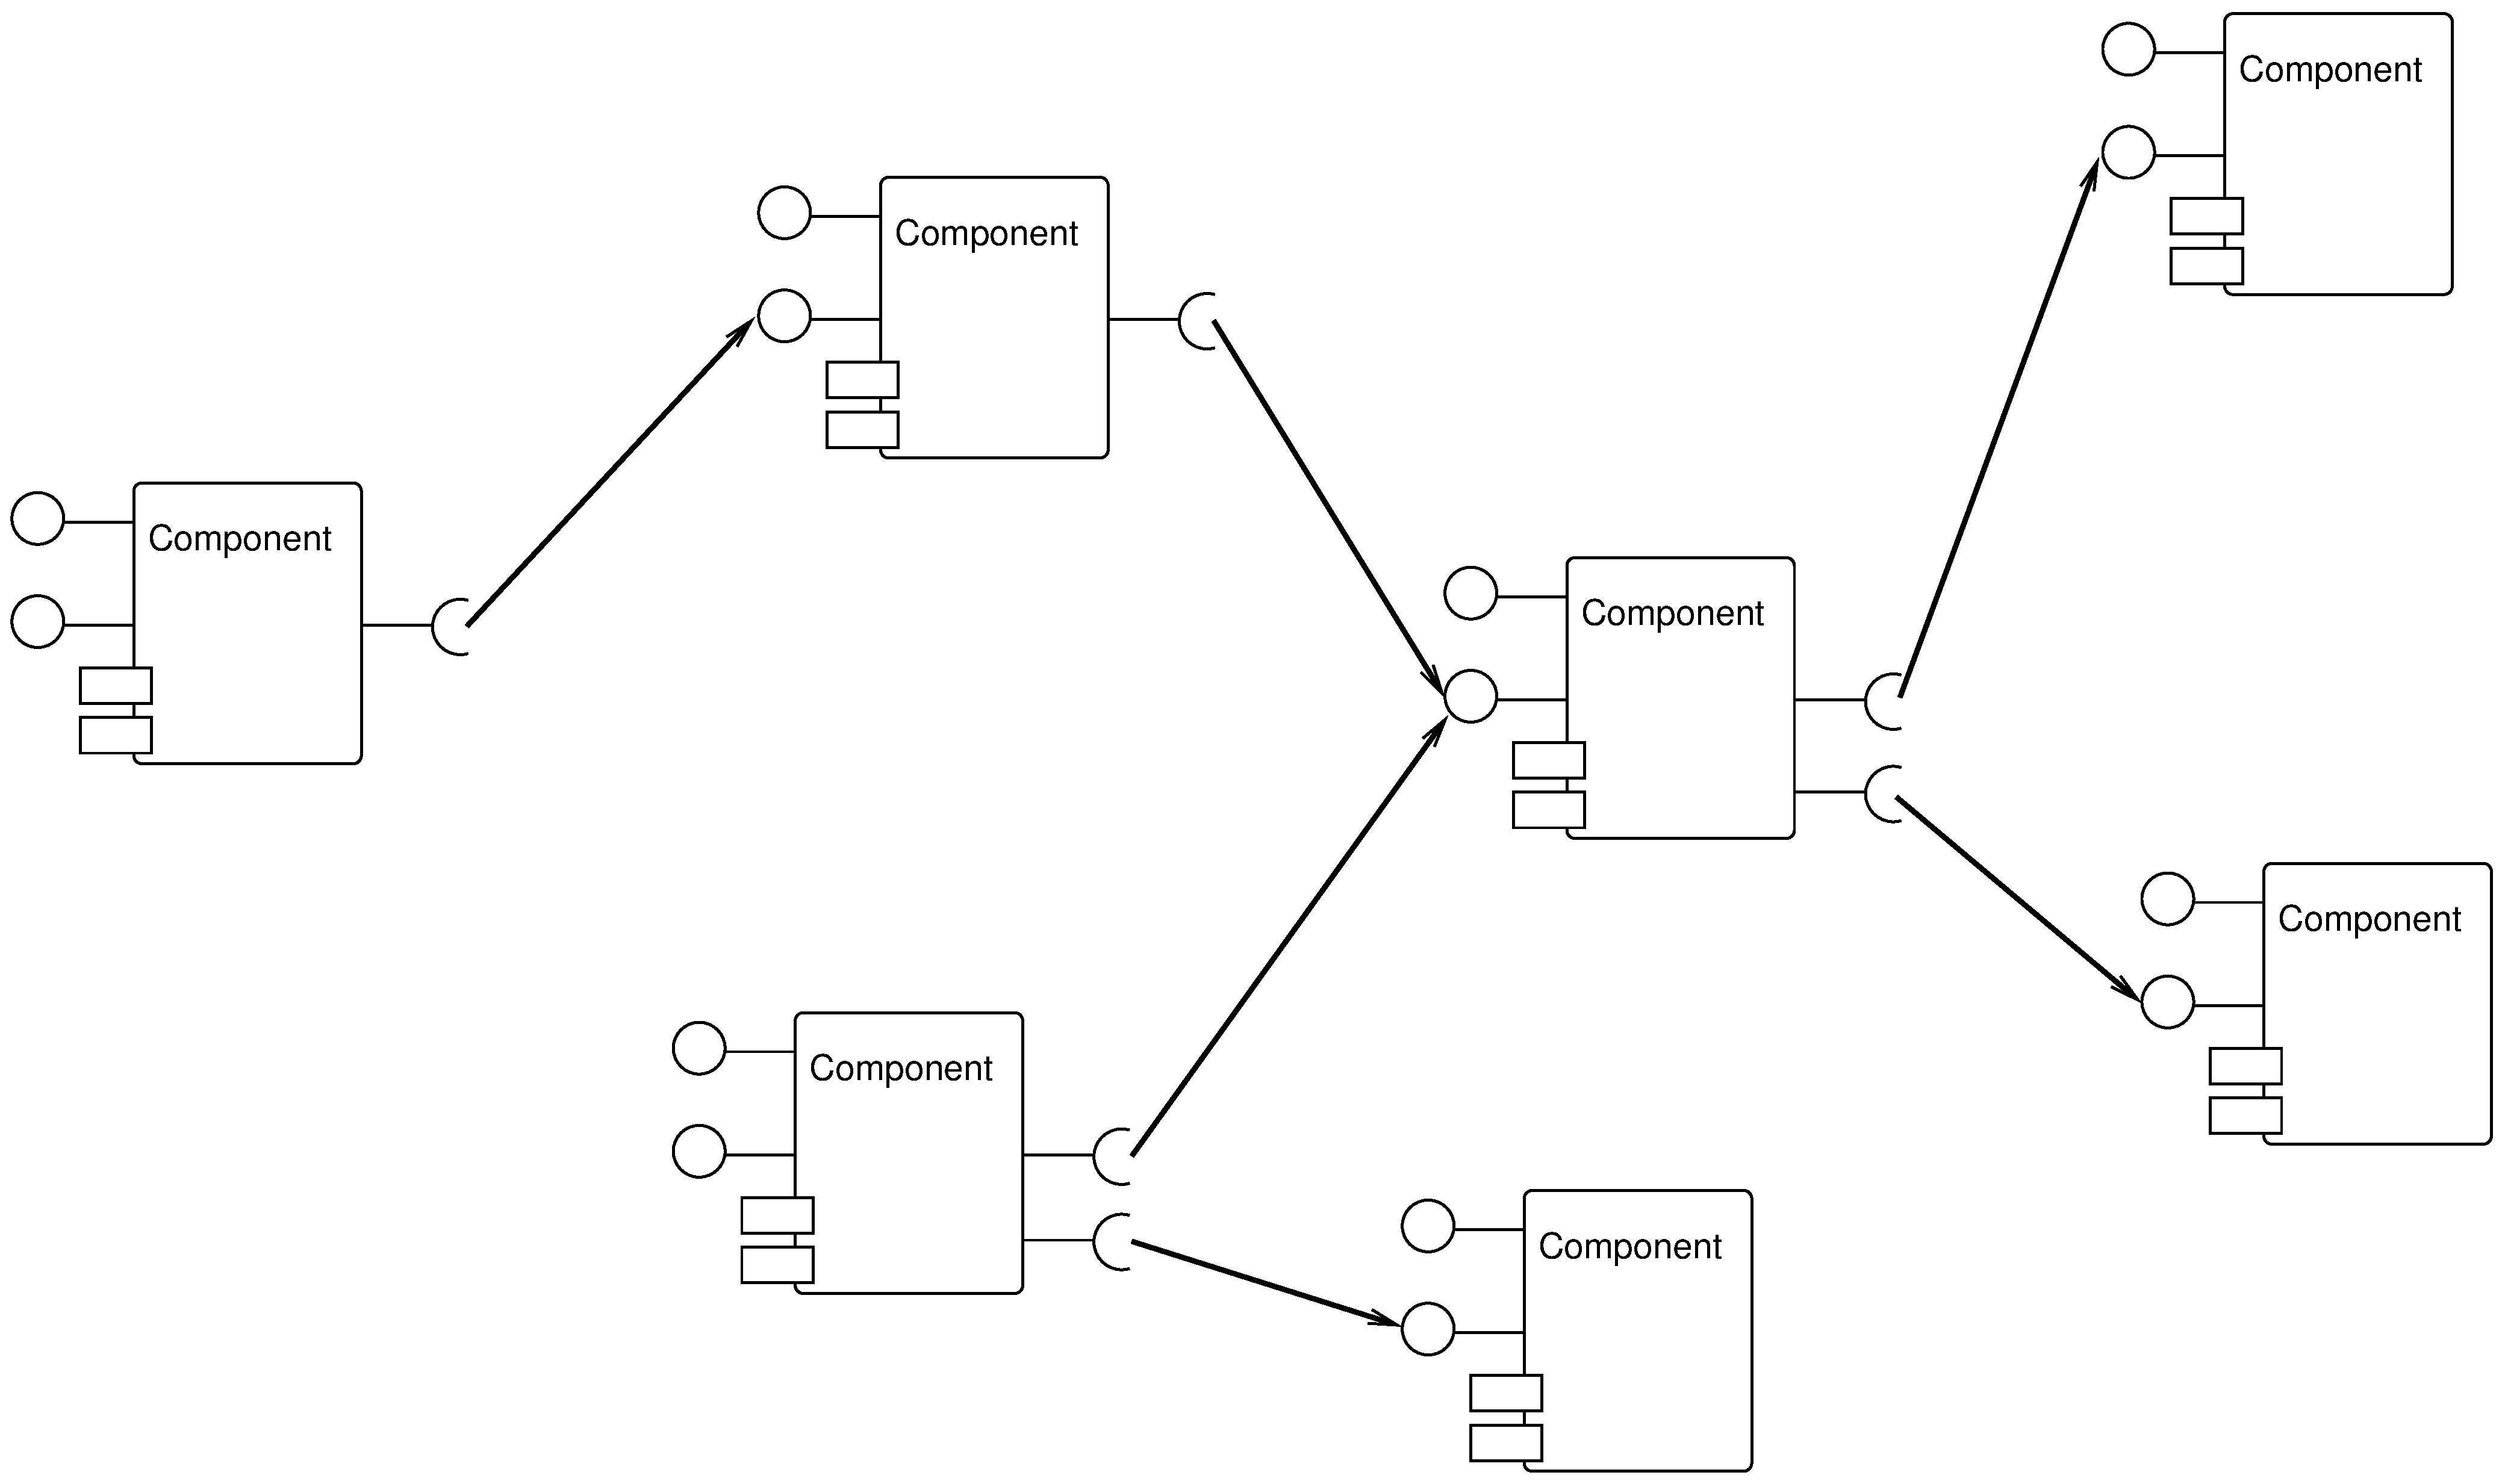
\includegraphics [width=10cm,angle=0] {figures/Assembly}
        \caption{Component assembly}
        \label{assemblygraph}
    \end{center}
\end{figure}

\noindent
The CCM assembly concept allows the creation of assemblies only at deployment 
time.
At runtime, a single component can not connect itself to another component.




\newpage
%==============================================================================
\section{Light Weight CORBA Component Model (LwCCM)}
%==============================================================================

Many of today's embedded CORBA applications are unable to use the available 
enterprise CCM due to design constraints.
These constraints include small code size in embedded environments and 
limited processing overhead for performance conservative applications.

\vspace{3mm}
\noindent
To overcome this problem, LwCCM
was submitted to the OMG \cite{LwCCM-Specification}.
The purpose of this profile is to specify a lightweight version of the CCM.
The principal aim of LwCCM is to have a component model sufficient to compose
applications with CORBA components without all optional features that are
not part of the ``core'' capabilities of CCM.
%This profile exposes what mandatory features should be contained in a 
%minimum implementation of the CCM. 
The choices made in the profile follow rules established to suit embedded
environments:
\begin{itemize}
\item {\bf Redundancy.}
If several ways of requesting a service exist, only one is retained.

\item {\bf Interoperability and Compatibility with full CCM.}
During deployment, a leightweight component should be deployable by a full
CCM deployment application. Connections between a leightweight component
and a full CCM component must be possible.
Implementations of leightweight components should be source compatible
with the full CCM.

\item {\bf Persistence.}
The LwCCM does not need to manage any kind of persistence as described in the
CCM specification. 

\item {\bf Transactions.}
Transactions are not a feature commonly used in embedded systems thus they
are not included in the LwCCM profile.

\item {\bf Security.}
Security will not be treated in the LwCCM profile.

\item {\bf Introspection.}
Not all introspection operations are retained in this profile because they
are not essential to perform the deployment of components.

\item {\bf EJB Integration.}
There is no integration of {\it Enterprise JavaBeans} defined in LwCCM
because EJB are not required for embedded targeted environments.

\item {\bf Deployment and Configuration.}
Instead of the {\it Packaging and Deployment} chapter of CCM, LwCCM
is based on the OMG {\it Deployment and Configuration} specification 
\cite{DeploymentAndConfiguration}.
This includes also the definitions of component and assembly descriptor
files and their XML DTDs.

\item {\bf CCM Implementation Framework.}
The whole {\it Component Implementation Definition Language} (CIDL) chapter 
as well as the {\it CCM Implementation Framework} (CIF) chapter are excluded 
from the LwCCM profile.

The CIDL is redundent with IDL definitions because all functional descriptions
of the component (facets, reseptacles, events and attributes) is done with the 
IDL files.
The way to assign a component category (service or session) to a component
can be done via an XML description file that will be used with the IDL files to
generate container code and skeletons.
\end{itemize}

\noindent
This profile tries to be as compliant as possible to the OMG 
{\bf Minimum CORBA} and {\bf Lightweight Services} specifications 
\cite{Minimum_CORBA, LightweightServices}.


